
\chapter{VUV measurement}
The measurement performed in this chapter were possible thanks to the network LaserLab, a consortium that brings together thirty institutions in laser-based disciplinary research from sixteen countries. In particular it was granted access to the CELIA beamline in Bordeaux.
CELIA (Centre Lasers Intenses et Applications) is a joint unit between the Universtity of Bordeaux, the CEA (Commissariat à l'énergie atomique et aux énergies alternatives) and the CNRS (Centre national de la recherche scientifique). It provides experimental access to femtosecond lasers at high frequency and VUV harmonics production.
The aim of the study is to characterize the rise time profiles of scintillating crystals at VUV energies.

As pointed out in chapter 5, the energy of the excitation of a fluorescent sample strongly influence the processes in the excitation region.
At the order of the band gap of the crystal, broadly speaking one photon is able to create a isolated electron hole-pair. As the energy of the excitation grows, more of this holes are created by a single quantum and different processes interact in the formation of the signal, such as electron–electron scattering.
As the erngy grows above hundreds of electron Volts, mainly core absorption occurs. 
Above a certain threshold Cerenkov events may allow to collect more photons at the risign edge of the signal. 
Investigation of interaction mechanisms requires sources with different energies and different geometries.
In this chapter a study with VUV radiation is presented. High-order harmonics generation by interaction of an intense laser field with atoms provides ultrashort pulses (2-3 ps) in the VUV (few tens of eV) region at high frequencies ($\geq$ 1 kHz). 
Under such pulse energy, a region of high excitation density is created in the crystal, since the photons interact in the first $\sym$ 100 nm of material.
Moreover the detector geometry will allow to focus the study on scintillator pulse, excluding any volume effect.

\section{High Harmonic Generation}
When an atom is exposed to a strong laser field it can absord a large number of photons through non linear processes. This energy can be transferred back to the photon field.
The phenomenon of high order harmonic generation of a laser field is a nonlinear effect that results in the emission of photons of frequency multiple of the source frequency. For example a rare gas traversed by a sufficiently power laser field may give rise to harmonic generation.
\begin{figure}[htbp]
\begin{center}
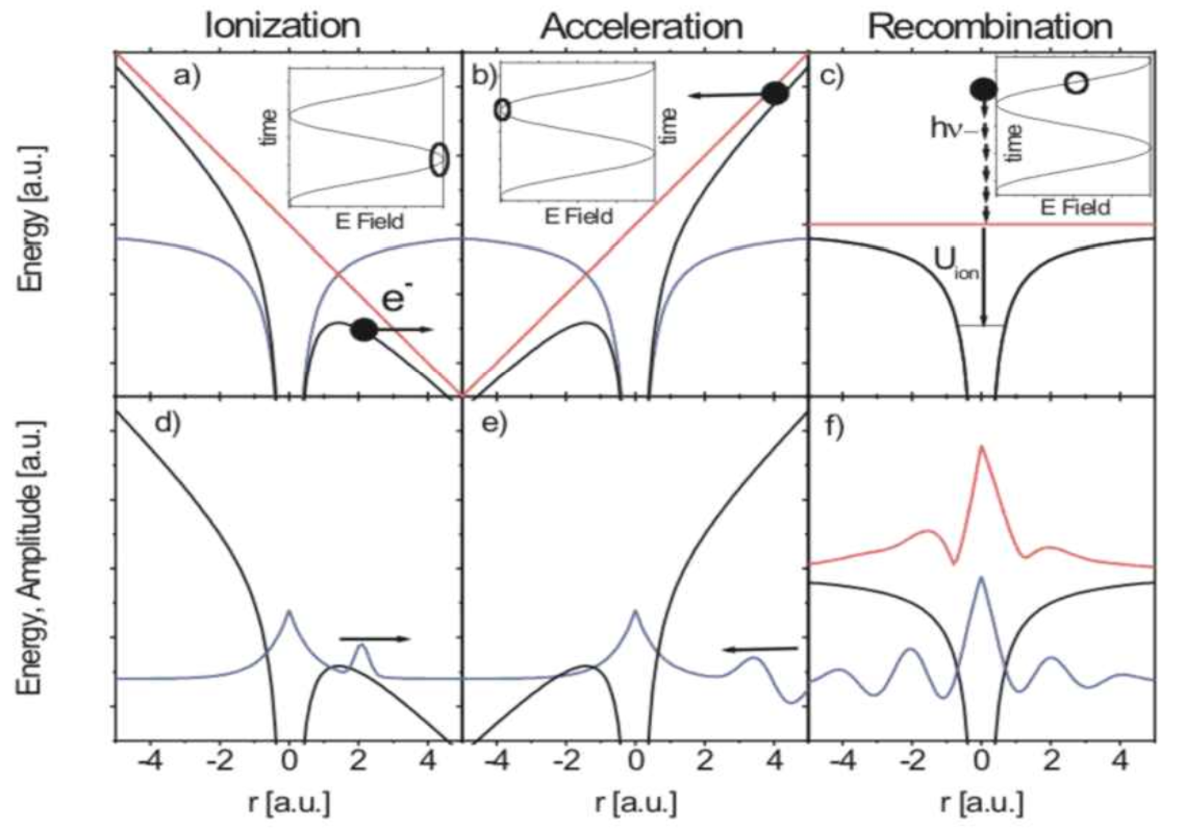
\includegraphics[width=12cm]{../Pictures/Chapter_7/HHG}
\end{center}
\caption[HHG phenomenology]{Phenomenology of High Harmonics Generation}
\label{fig:HHG}
\end{figure}

In figure \ref{fig:HHG} the main details of the high harmonic generation process are summarized, in a semi-classical configuration and as a quantum wave process.
If the laser field is strong enough ($\sim 10^{10}$V/m), it can allow the electron to tunnel through the barrier. The electron itself sits unperturbed in the well until the field of the laser sums to the atom potential bending it.
The electron gets accelerated in the laser field and it can recollide with the atom itself. The electron kinetic energy is then transferred into photons.
The cut-off energy can be calculated by examining the maximum energy the ionized electron can gain in the electric field of the laser, that is
\begin{equation}
E_{max} = I_{p}+3.17U_{p}
\end{equation}
where $U_{p}$ is the ponderomotive energy from the laser and $I_{p}$ is the ionisation potential. The recollision leads to the emission of a very broad light spectrum.
The ionization and recollision happen on each half cycle of the laser pulse, and the spectra are added coherently. As a consequence the spectrum is structured in odd harmonics.
High harmonics constitute a source of soft X-rays that retains the time characteristics of the driving laser, in terms of bunch structure and repetition rate. 
The harmonic cut off varies with the laser intensity up to saturation. The saturation intensity depends on atomic species of the noble gas used as a medium to produce the harmonics.

\section{Experimental setup}
The setup available at CELIA it is presented in \cite{Martin2001}. it will be briefly described here. The line is organized in two different room. A first room is devoted to the laser amplification system, while in the experimental room the high harmonics are produced.
\subsection{Laser beamline}
The AURORE beamline is based on a amplified Ti-sapphire femtosecond oscillator. 
The Ti-sapphire oscillator generates 30 fs pulses, at 1 nJ and a frequency of 80 MHz. Before amplification the pulses are stretched up to 280 ps for optical power reasons.
The regenerative pre amplifier brings the energy of the beam to 700 $\micro J$ at 1 kHz.
The beam is then amplified in a Ti:sapphire crystal pumped by four synchronised Nd:YLF lasers at 532 nm and 15 W.
At the end of the amplification chain the laser beam delivered has a power of 10 W for 170 ps and it is sent to the experimental room.
%figura laser
\subsection{VUV line}

\begin{figure}[htbp]
\begin{center}
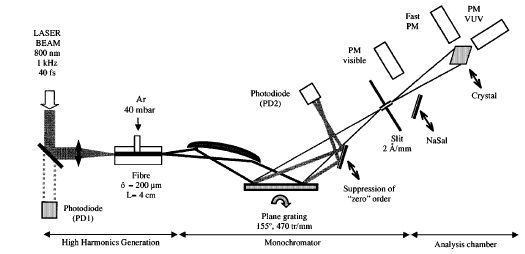
\includegraphics[width=12cm]{../Pictures/Chapter_7/VUV_line.png}
\end{center}
\caption[VUV line]{Schematics of the VUV line at CELIA Bordeaux}
\label{fig:VUV_line}
\end{figure}
Before high harmonic generation the beam is compressed again down to 35 fs, centered around 800 nm at 1 kHz, with an energy of 4 mJ.
A schematic of the HH VUV beamline is presented in fig
The elements are under vacuum at a pressure of $10^{-6}$ mbar. The beam is focused in the fiber containing the gas (200$\mi m$ in diameter and 4 cm length). Depending on the gas used and the pressure condition the energy of the harmonic lines and the efficiency of the process may vary. Tipically in Argon/Neon the energy of the harmonics is between 10 eV and 120 eV.
The fundamental beam and the harmonics spread at the exit of the fiber and are sent to the monchromator where a toroidal mirror and a plane grating (470 lines/mm) focuse the selected wavelength on the exit slit.
The zero order is suppressed by a plane mirror at an angle tuned on the grating system.
The desired VUV-XUV beam selected in energy is then directed to the sample placed in a vacuum chamber. Due to the dispersion by the grating the output pulses are stretched in time, and they have been measured with a VUV-streak camera to be 2-3 ps FWHM.

\subsection{Detection system}
The light produced by the luminescent sample hit by the VUV-XUV radiation is collected by an optical fibre visible-UV of 0.6 mm diameter mounted on a side of the chamber and connected to a monochromator (TRIAX Jobin-Yvon 130) by a focalisation system.
The monochromator is equipped with three diffraction gratings, one with 1200 lines/mm and the others with 300 lines/mm. This allows to cover a spectral range between 200 nm and 1000 nm.

%The emission spectrum is measured by mean of a CCD camera 
%manca il modello!
The photon counting device is a Hamamatsu MCP-PMT R3809U-52 model. The DAQ system is shown in figure \ref{fig:daq}.
The signal from the laser trigger is routed into a Ortec Pico Timing Discriminator (model 9307). A first output is directed directly to a Ortec Time to Analog Converter (model 9308).
A second output is directed to a Lecroy Quad Coincidence Unit (model 622).
The MCP-PMT signal is preamplified by a ORTEC 1-GHz preamplifier (model 9306) with a gain of 100 and then sent to a second Pico Timing Discriminator. One output is sent to the Lecroy Quad Coincidence Unit and a second one delayed by 60 ns and sent to the TAC. The last unit is required since the laser trigger has a fixed delay. 
A third output is sent to a SR400 Gated Photon Counter (Stanford Research System) along with the output of the Lecroy coincidence unit.
The SR400 Gated Photon Counter allows to determine the rate of counts at the MCP detector, to keep under control the fraction of biased events.
The TAC guarantees a 16-bit digital resolution in the range 0-325 $\micro$s down to a binning of 1.22 ps and its signal is sent to a computer for the software system to finally determine the delay between the MCP and the laser trigger.
\begin{figure}[htbp]
\begin{center}
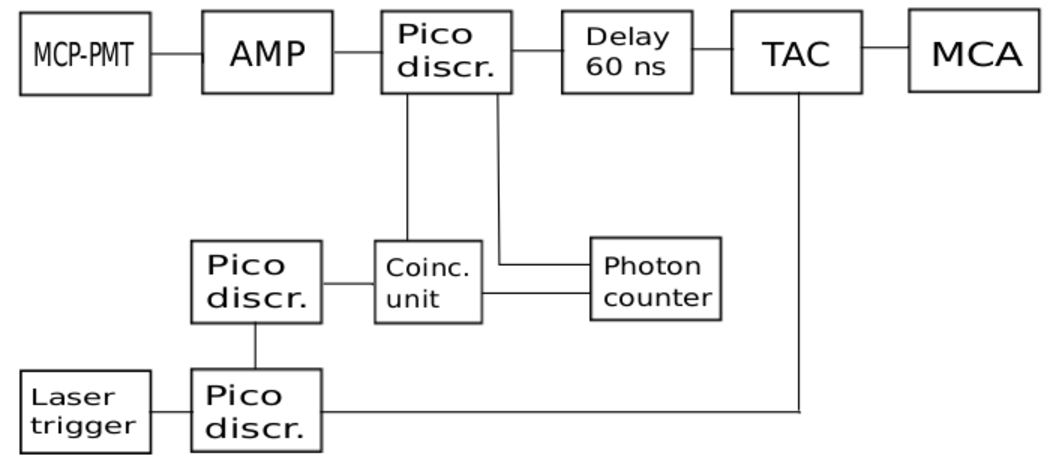
\includegraphics[width=9cm]{../Pictures/Chapter_7/electronics.pdf}
\end{center}
\caption[VUV DAQ]{Schematics of DAQ system}
\label{fig:daq}
\end{figure}

\section{Preliminaries}
Three parameters have to be kept under control during the irradiation, as they influence the sistematics of the system:
\begin{itemize}
\item energy of the excitation
\item impulse response function of the system
\item laser stability and photon counts
\end{itemize}

\subsection{VUV spectrum}

In Fig. 2, we show the harmonic spectra of six harmonics in
argon ( 40 mbar) between 28 and 47 eV. These spectra were
obtained in the same conditions of spectral resolution but with
different intensities of the fundamental laser beam. The intensities
of the 800-nm laser beam at the entrance of the fiber are,
respectively, about 1, 2, and 4 mJ for spectra (a), (b), and (c).
At low intensity, the emission spectra of harmonics is characterized
by narrow peaks; at intermediate intensity, the shape of
each “ band” is complex with a blue shift of narrow peaks and
the appearance of a large pedestal. The experimental spectrum
(c) measured with the highest intensity shows large bands with
an important overlapping.
The HH spectra are controlled by the electron trajectories of
each excited argon atom electron with different return time [14].
Anarrowpeak can be attributed to the emission of electrons with
return time of less than half a laser period. HH radiation with a
large pedestal is connected to the emission of electron with return
time close to a full period of the laser field and has a larger
divergence. As mentioned above, it is clear that in these conditions,
the HH emission spectrum is a quasi-continuous one.

\begin{figure}[htbp]
\begin{center}
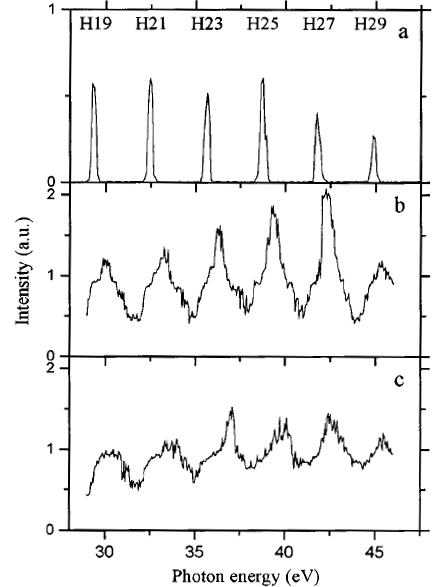
\includegraphics[width=7cm]{../Pictures/Chapter_7/VUV_spectrum.png}
\end{center}
\caption[VUV spectrum]{Schematics of the VUV line at CELIA Bordeaux}
\label{fig:VUV_spectrum}
\end{figure}

\subsection{IRF measurement}
The Impulse Response Function (IRF) is the response of the DAQ system to a narrow excitation in time. This is usually measured at the beginning of the campaign and checked for stability at regular intervals.
In this specific setup the width of the exctitaion pulse can be substantially neglected, being an order of magnitude below the typical scale of the pyshical processes involved. Thus the main sources of fluctuations in the timing response are the TTS of the photo detector and the electronics.

In order to quantify the IRF, the standard procedure is to directly hit the photodetector with the laser light and measure the delay spectrum with respect to the trigger signal of the laser.
If we consider the jitter on the trigger negligible, as it is in most cases, the only parameter to keep under control is the number of counts of the photo detector. 
In order to retain a low probability for pile up, the SR400 Gated Photon Counter was kept under control, well below 100 counts on a 1-second gated window. 
The IRF for the system is shown in figure \ref{fig:IRF}
\begin{figure}[htbp]
\begin{center}
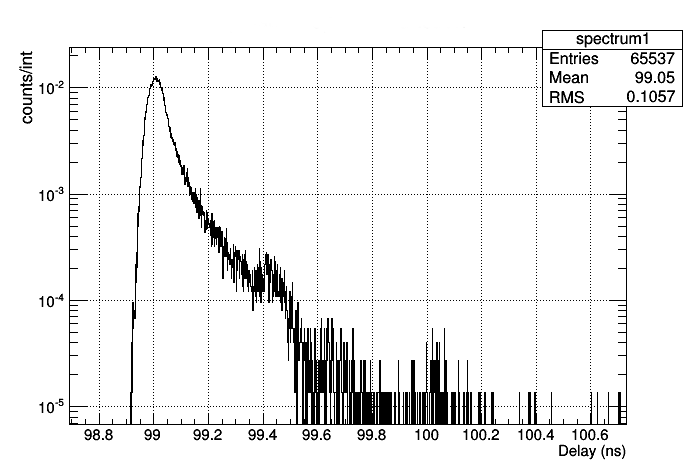
\includegraphics[width=6cm]{../Pictures/Chapter_7/IRF_simple.png}
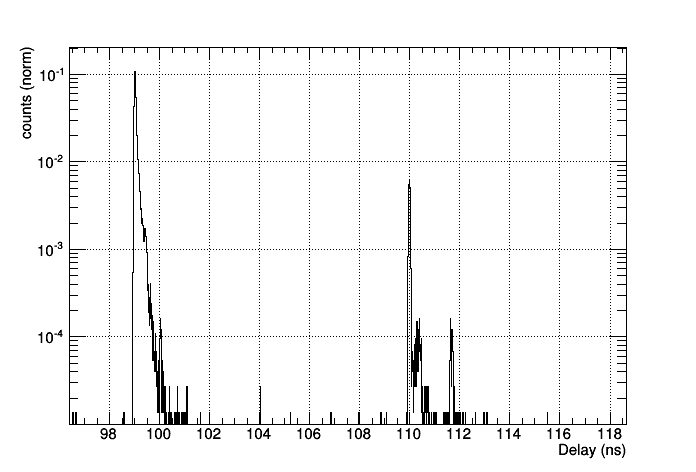
\includegraphics[width=6cm]{../Pictures/Chapter_7/long.png}
\end{center}
\caption[VUV setup IRF]{Impulse Response Function of the system excitation VUV - MCP-PMT.}
\label{fig:IRF}
\end{figure}
The IRF of the system, modeled with a multi Gaussian with tail towards high times due to ion feedback, gives $\sigma _{IRF} = $ 30 ps.
In particular two parameters should be considered in terms of degradation of resolution: the width of the response under the first tailed Gaussian, and the ratio between the first peak and the ion feedback delayed one (in this case this delay amounts to $sim$ 350 ps). In this case two order of magnitude separates the main and the secondary peaks.
As shown in figure \ref{fig:IRF} the IRF shows a reflection, which is not eliminable because the setup could not be modified for logistics reasons. This is never a nuisance for very fast cinetics, but it makes accurate decay time measurements for long decays not feasible. For rise time measurement this is not limiting, since the range can be safely tuned to extract the parameters, as will be shown below. 

The measured IRF is deconvoluted from the measured signal via the method described in the previous chapter.
This value accounts for three effects which can not be disentagled: the noise level of the instrumentation with rapport to the height of the signal, the TTS of the detector and the time walk of the detector itself.
As will be shown in the next chapter Hamamatsu MCPs present a large amount of time walk jitter, which can not be corrected in this setup. Considering a signal that ranges from 5 mV to 50 mV for single photons, and the amplification gain of the Ortec pre amplifier ($sim$ 100), the signal from the Ortec pico timing discriminator suffers from a $\geq\pm$20 ps shift in the timing output for the range considered.
This is in agreement with the data from the producers, since the time walk corrected MCP nominal $\sigma _{SPTR}$ is $\sim$ 20 ps and the laser contribution (2-3 ps FWHM) can be neglected.

\subsection{Control of the bias fraction}

As discussed in the previous chapter, the count rate at the stop detector bias the measurement at high pile up probability. In the case of a MCP-PMT the probability of pile up is still very low ath the typical time constants of the samples measured, since the dead time of the detector is less than 1 ns. 

There is no direct way to store the actual pulse that is fed to the electronics in this setup, so it is necessary to completely rely on the values given by the SR400 Gated Photon Counter. 
This device allows to control dinamically the number of pulses fed to the electronics on a given time window, which is usually set to 1 s. Knowing the typical time constants of the sample in exam, or checking it with a quick preliminary measurement, allows to choose an appropriate number of counts per second, which is for all the samples measured between 100 and 200 Hz.
In the case of rise time, as shown in the previous chapter the effect of high count rates is less pervasive on the parameter extracted, and at the rates considered in this VUV setup does not affect the values obtained significatively.

% plot di differenza ( quelli che avevamo fatto a diversi conteggi)
% ma anche no
%\subsection{Preliminary measurements}
% la voglio?

\section{Data analysis}
The samples masured present different size and surface condition in terms of polishing and depolishing.
Nevertheless this aspects can be neglected, given the excitation energy and the geometry of the setup.
Indeed photons in the VUV range, as already discussed, can travel for very short distances in a heavy scintillator, in the range of one hundred of nanometer. This means that the excitation takes place on the surface of the crystal. Nevertheless of the radiation comes on the opposite side of the detection system, one could not neglect transit time effect of photon extraction. The geometry of the system is shown in figure \ref{fig:geom}: an optical fiber is able to collect photons coming directly from the excitation point on the surface, that is photon extracted at higher angle and thus rebounced at the lateral faces will be highly suppressed at the detector.
\begin{figure}[htbp]
\begin{center}
\includegraphics[width=7cm]{../Pictures/Chapter_7/}
\end{center}
\caption[]{}
\label{fig:geom}
\end{figure}
The samples measured were:
\begin{itemize}
\item LSO:Ce,Ca (2x2x3 mm$^{3}$) 
\item LSO:Ce (CTI, 2x2x3 mm$^{3}$)
\item LYSO:Ce (Proteus, 2x2x3 mm$^{3}$)
\item LYSO:Ce (Sipat, 2x2x3 mm$^{3}$)
\item LGSO:Ce (2x2x3 mm$^{3}$)
\item CeF$_{3}$ (2x2x3 mm$^{3}$)
\item LuAG:Ce (0.13$\%$, 2x2x3 mm$^{3}$)
\item LuAG:Ce (0.08$\%$, 2x2x3 mm$^{3}$)
\item LuAG:Ce (0.5$\%$, 2x2x3 mm$^{3}$) 
\item LuAG:Ce (0.44$\%$, 2x2x3 mm$^{3}$)
\item LuAG:Pr (1.5x1.5x3 mm$^{3}$)
\item BGO (3x3x5 mm$^{3}$)
\end{itemize}
%2739, 2408, 2737, 2445, 2583, 2741, 2735, 2609, 2612, 2611, A3, A1
% quali problemi riscontrati (parlo della riflessione risposta? si, se parlo del decay == stand by)
% influenza IRF andare a recuperare i plot
% different binning
% statistica
Due to time constraints, measurements were performed at a 1 ps TDC binning for crystals with high light yield. For crystals with low light yield (almost all the Garnets), the binning was increased to 10 ps, at the expenses of limited accuracy.
\section{Fit procedure}
The fit procedure has been presented in the last chapter and it consists in the minimization of the function $-\log{L}$, where the likelihood function $L$ has been defined in the previous chapter and is given by the convolution of the model and the IRF.
The function used for the fit is a simple multi-exponential model for n decay component as
\begin{equation}
p(t) = \sum _{i = 1}^{n} \frac{P_{i}}{\tau _{d, i} - \tau -{r, i}}\left( e^{-\frac{t-t_{shift}}{\tau _{d}}} - e^{-\frac{t-t_{shift}}{\tau _{r}}} \right) + C_{bg}
\end{equation}
and $\tau _{shift}$ is the turn-on of the scintillation pulse and $C_{bg}$ is the background level.
The software used for minimization is Matlab.

In order to determine the confidence interval on the parameters it is necessary to consider the influence of three parameters on the fit results, that is the rise time, the decay time and the range of the fit. 
The number of counts collected for the spectrum 
We consider here only the case for one single component, in the case of rise time is usually enough to consider the first component, especially if it is significatively longer than the rise time constant. This is the case for most of the samples measured: as an example the LSO cerium doped compounds present a rise time of the order of $\sim$ 50 ps and a decay time of the order of $\sim$ 40 ns.
In order to quantify the effect of mutual variation of fit parameters, a simple toy model was used with the shape described above. The analysis was then performed over the samples measured for parameters estimation.

The range of the fit sistematically influences the time constants extracted. As the range considered is enlarged, the  decay part of the spectrum becomes more relevant, and artefacts in the IRF influence the parameters extracted. 
It is then necessary to restrain the range of the fit, since the IRF measured for the setup presents reflections at longer times. On the other hand restricting the range  entails a loss of information for what concerns the decay part of the curve. In a first time we are not interested in defining the decay time with the best possible accuracy, so we chose a range that optimizes the rise time determination.

The toy model used presents in this case a rise time of 36 ps and a decay time of 33 ns. 
In order to quantify the effect of range variations on the fit, we let the range itself free over significative bins, that is starting from the rise of the scintillation pulse.
In figure \ref{fig:range} is shown the influence of range variation on the extracted parameters form the fit routine.
For what concerns the decay time, as soon as the range start to comprehends a larger fraction of the decay of the pulse, the value stabilizes and the change is contained in less than 5 ns variation which is optimal considering the likelihood confidence level. There is a sistematic under estimation of the value, though, since the loss of indormation on the last part of the pulse bias the fit routine, as shown in previous chapter.
The same goes for the rise time in terms of comparison with the likelihood confidence level, therefore the optimal range was chosen to be over bin 15000. In this configuration the influence of the range is limited to a few ps.
\begin{figure}[htbp]
\begin{center}
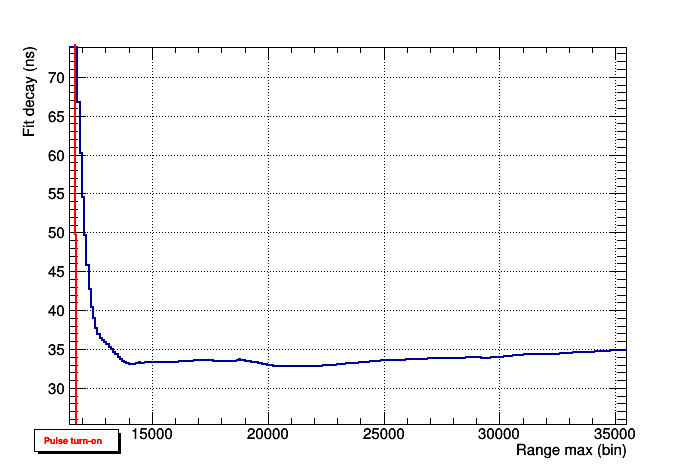
\includegraphics[width=6cm]{../Pictures/Chapter_7/decay_range_2.png}
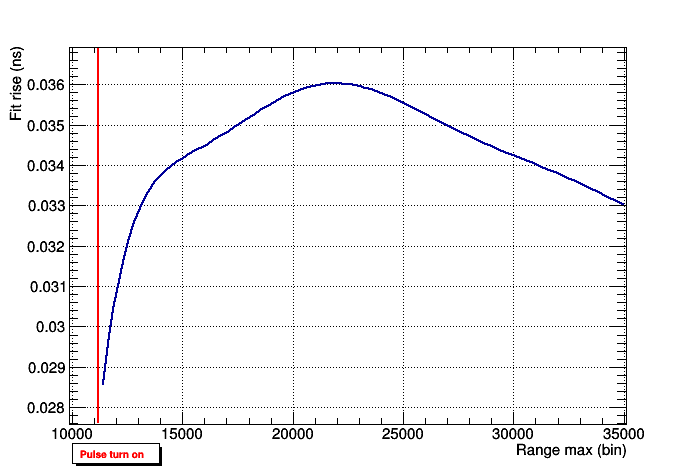
\includegraphics[width=6cm]{../Pictures/Chapter_7/rise_range_2.png}
\end{center}
\caption[]{}
\label{fig:range}
\end{figure}

For what concerns the confidence level on the parameters extracted from the fit, we profiled the two dimensional likelihood over the parameters optimized, that is rise time and decay time, as shown in figure \ref{fig:likelihood} for different number of counts collected for the rise time.
In this case a binned likelihood approach requires a determination of a confidence interval based on a asymmetric likelihood.
At the best fit point the function to minimize  $-2\ln{L}$, tends to a chi-squared distribution for (n-2) degrees of freedom. In this case it is customary to define a confidence level the interval ($min_{L}$, $min_{L}+\frac{1}{2}$) since in the limit of normally distributed data for large counts it translates to a 95$\%$ confidence level. In this case the likelihood is close to this approximation, therefore this convention will be used for confidence intervals.
\begin{figure}[htbp]
\begin{center}
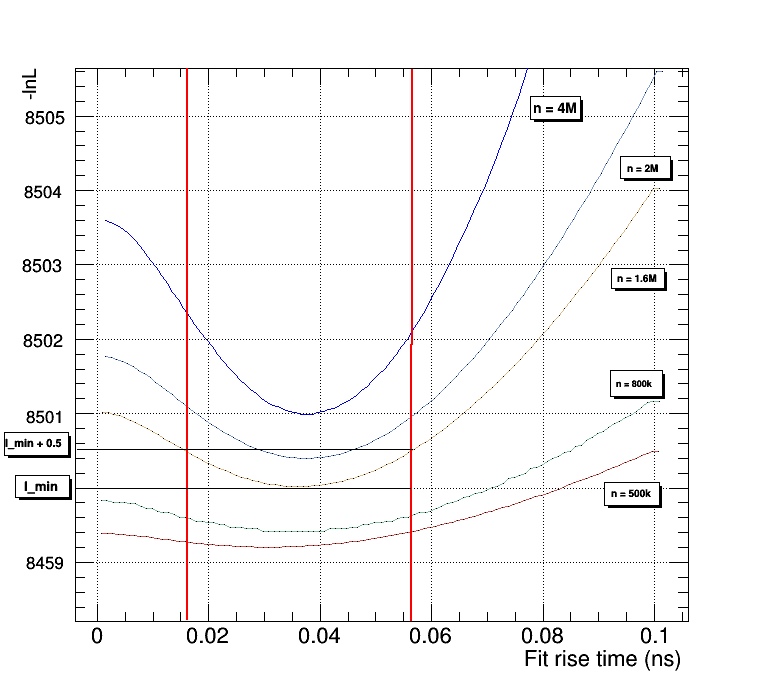
\includegraphics[width=6cm]{../Pictures/Chapter_7/error_rise.png}
\end{center}
\caption[]{}
\label{fig:likelihood}
\end{figure}

As an example in figure \ref{fig:likelihood_sipat} the case for a LSO Sipat crystal is shown. In this case, for a bi exponential fit with one component decay, we will quote the values, with relative asymmetric confidence level $\tau _{r} = 36_{-30}^{+27}$ ps and $\tau _{d}40.5_{-0.9}^{+0.7}$.
\begin{figure}[htbp]
\begin{center}
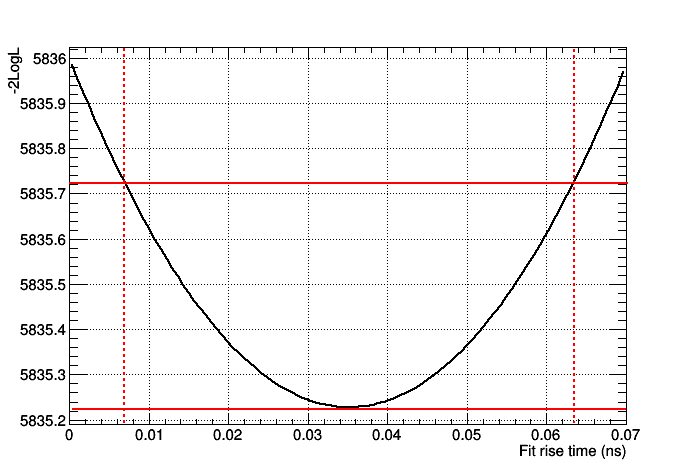
\includegraphics[width=6cm]{../Pictures/Chapter_7/rise_sipat.png}
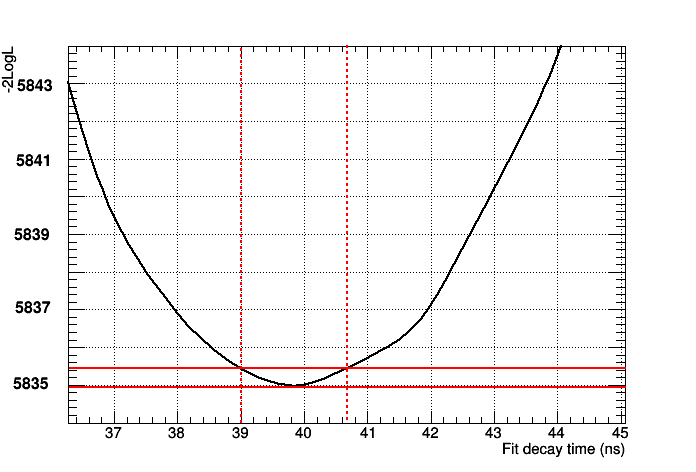
\includegraphics[width=6cm]{../Pictures/Chapter_7/decay_like_2.png}
\end{center}
\caption[]{}
\label{fig:likelihood_sipat}
\end{figure}

\section{Results}
\subsection{Data}
The results obtained for the sample measured can be boradly divided in two groups: a first group contains the LSO type crystal, the CeF$_{3}$ and the BGO and they present very fast rise times ($<$ 40 ps).
The group of the Garnets, on the other hand, with different dopings (Ce and Pr), presented slower rise times ($>$200 ps).
Plot for the different samples measured are shown in the figures of this section. On the top, the deviance residuals obtained for likelihood estimation, to graphically show large bias in the fit data if present. This residuals are defined as
\begin{equation}
R_{i} = \sqrt{2\left[ c_{i}\log{\frac{c_{i}}{g_{i}}-c_{i}+g_{i}} \right]}sign\left[ c_{i}-g{i} \right]
\end{equation}
and $c_{i}$ and $g_{i}$ are respectively the counts and the model expectations in channel i.
The values obtained for the decay time, as discussed in the previous section, should be considered carefully. 
Since our main interest does not lie in the decay time and given the problems related to the IRF, the range of the fit was restricted. This leads to a sistematic under estimation of the decay time.
% eventualmente aggiungere qualcosa su laser / x-ray
For the case of Sipat LYSO, Proteus LYSO, CTI LSO and LGSO,  the parameters were extracted considering a one component decay. 
% eventualmente dire qualcosa su laser/x ray
For what concerns CeF$_{3}$ and LSO:Ce,Ca the fit was performed for a two decay component curve. This is in agreement with measurement performed in this study (see next chapter), in \cite{Gundacker2014}, and in \cite{ref:Lecoq2006}.
It is worth to underline that in this case, as the first fit component is quite fast ($<$10 ns) the value is more accurate, since accuracy benefits from a larger time window.

\begin{figure}[htbp]
\begin{center}
\includegraphics[width=7cm]{../Pictures/Chapter_7/}
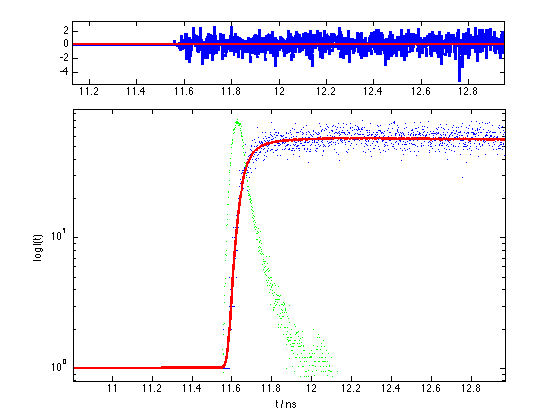
\includegraphics[width=7cm]{../Pictures/Chapter_7/2737_proteus.png}
\end{center}
\caption[LYSO Sipat profile]{}
\label{fig:sipat_proteus}
\end{figure}

\begin{figure}[htbp]
\begin{center}
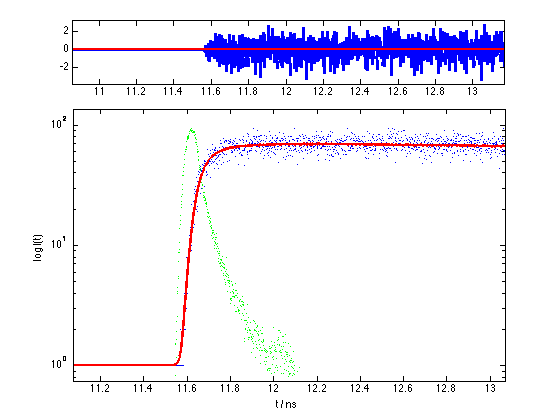
\includegraphics[width=7cm]{../Pictures/Chapter_7/CTI.png}
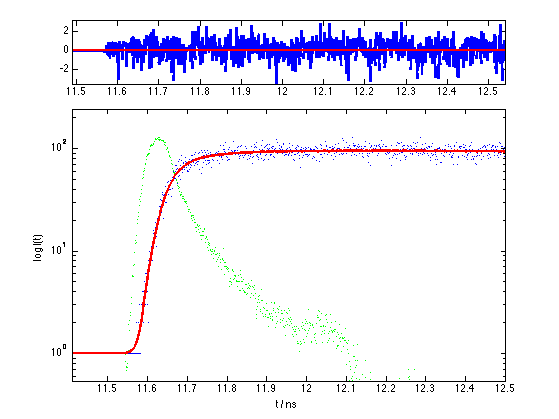
\includegraphics[width=7cm]{../Pictures/Chapter_7/ca_ce.png}
\end{center}
\caption[]{}
\label{fig:cti_cace}
\end{figure}

\begin{figure}[htbp]
\begin{center}
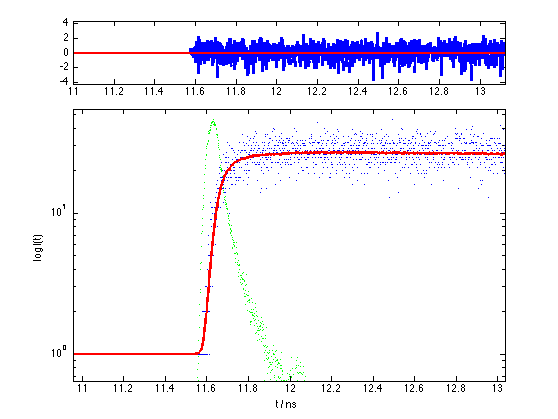
\includegraphics[width=7cm]{../Pictures/Chapter_7/lgso.png}
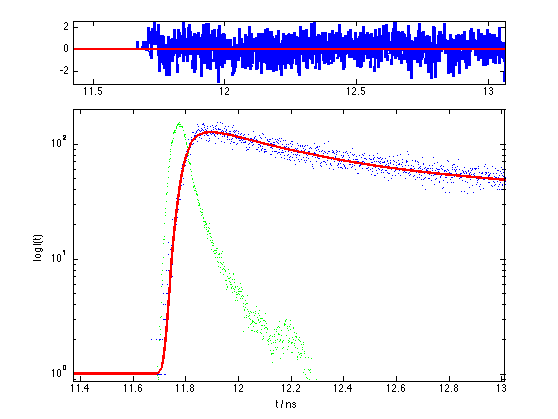
\includegraphics[width=7cm]{../Pictures/Chapter_7/cef3.png}
\end{center}
\caption[]{}
\label{fig:lgso_cef3}
\end{figure}

\begin{figure}[htbp]
\begin{center}
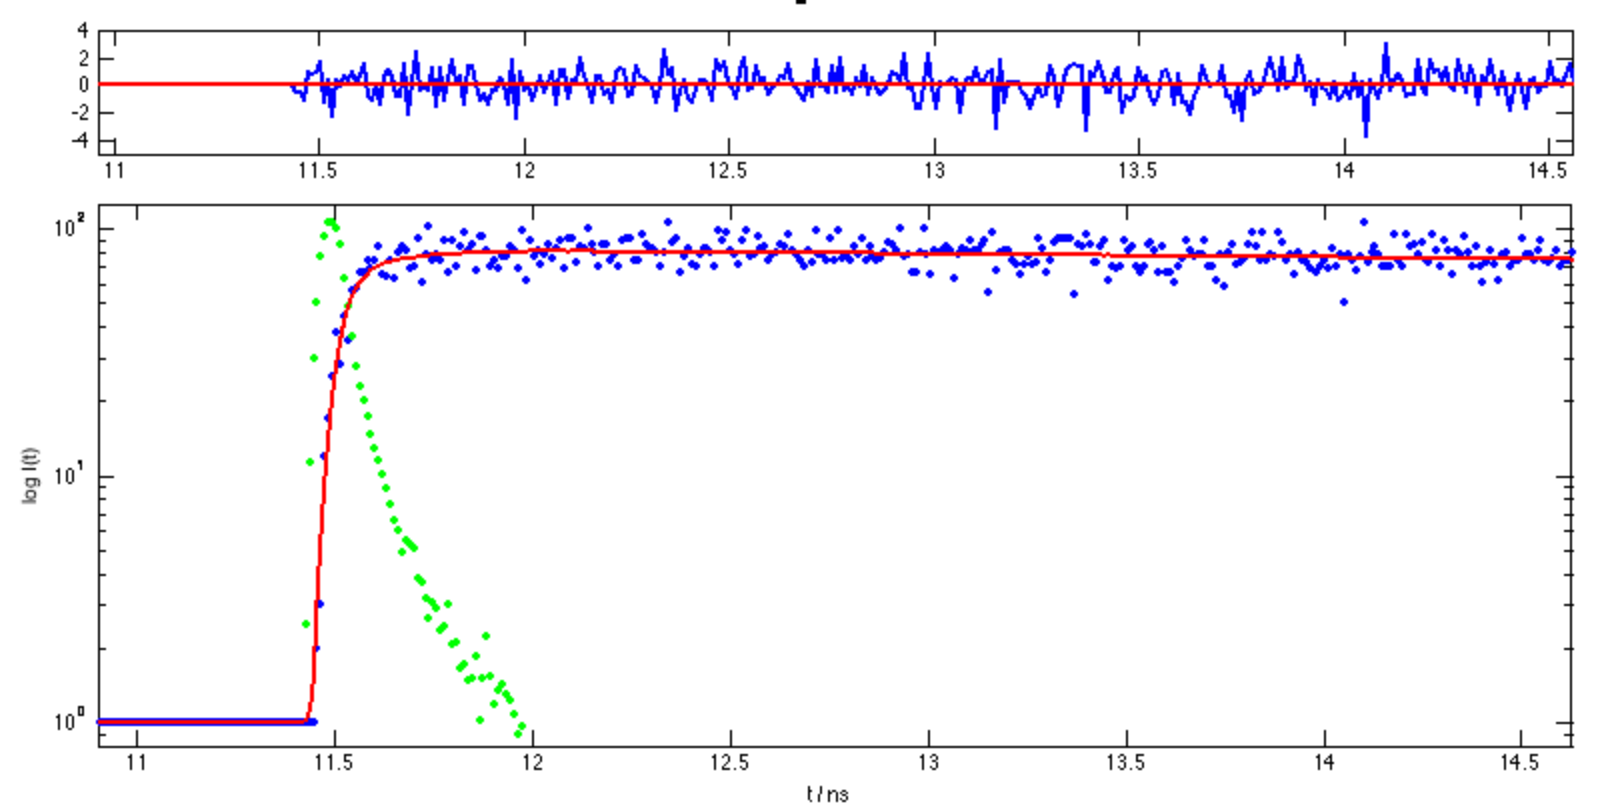
\includegraphics[width=7cm]{../Pictures/Chapter_7/bgo.png}
\end{center}
\caption[]{}
\label{fig:lgso_cef3}
\end{figure}

\begin{table}[h]
\begin{center}
\begin{tabular}{llll}
Crystal  & $\tau _{r}$ & $\tau _{d, 1}$ & $\tau _{d, 1}$ \\
LYSO Sipat      & 36_{-27}^{+30} ps         & 40.5_{-0.7}^{+0.9} ns  & \\
LYSO Proteus     & 26_{-26}^{+30} ps         & 39_{-0.7}^{+0.9} ns & \\ 
LSO CTI      & 23_{-18}^{+20} ps         & 37_{-0.8}^{+0.8} ns  & \\ 
LSO:Ca      & 23_{-19}^{+22} ps         & 10_{-0.3}^{+0.4} ns  & 30_{-0.8}^{1.0} ns \\ 
LGSO & 27_{-15}^{27} ps         & 38_{-0.8}^{+0.8} ns & \\  
CeF$_{3}$      & 22_{15}^{30} ps         & 5_{-0.2}^{+0.4} ns  & 18_{-0.5}^{+0.8} ns \\
BGO      & 30_{25}^{35} ps         & 10_{-0.2}^{+0.4} ns  & long
\end{tabular}
\end{center}
\label{table:table}
\end{table}

As briefly explained before, the measurements for some LuAG samples were performed with a different TDC binning, due to the scarce light yield that implied very long accumulation times. In these cases the tdc binning is 10 ps. As shown previously this influences the error on the rise time, which for these samples is more pronounced.
The Garnets show different time constants, and can vary very much based on the doping concentration, the purity of the sample, the energy of the excitation. Since the measurements are performed on a limited time window, the decay time can be quite biased towards fast constants, and very low decay times can be indistinguishable from background.
\begin{figure}[htbp]
\begin{center}
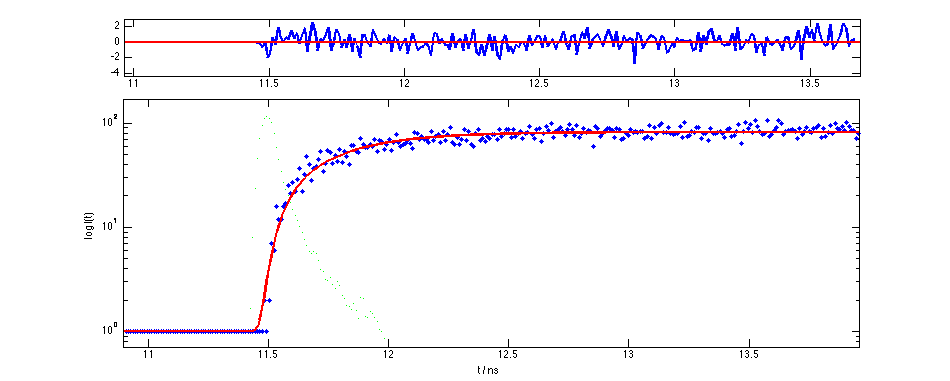
\includegraphics[width=7cm]{../Pictures/Chapter_7/luag_0_0_8.png}
\end{center}
\caption[]{}
\label{fig:luag_1}
\end{figure}

\begin{figure}[htbp]
\begin{center}
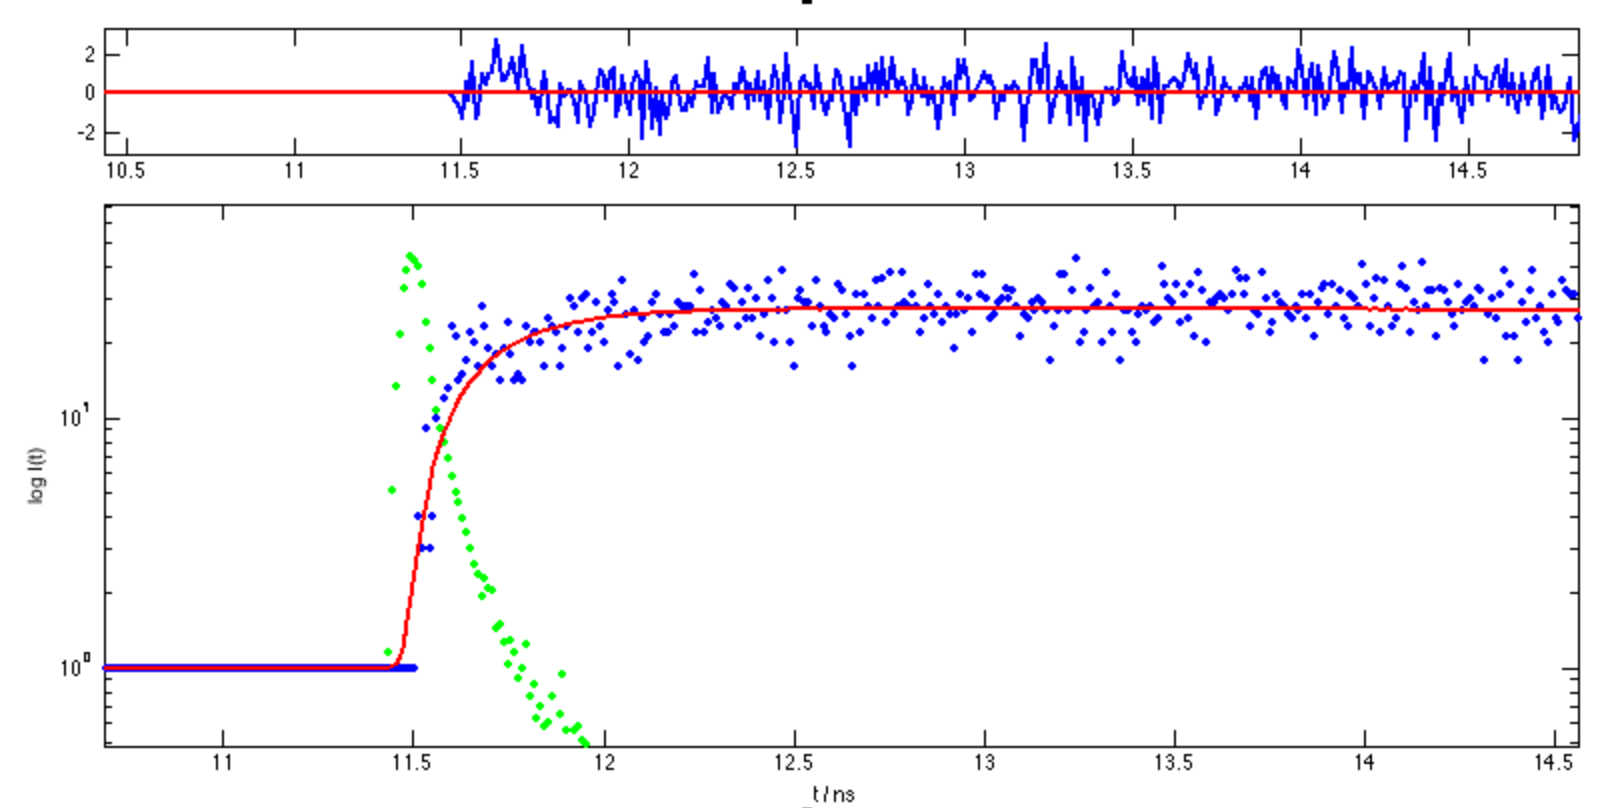
\includegraphics[width=7cm]{../Pictures/Chapter_7/2612.png}
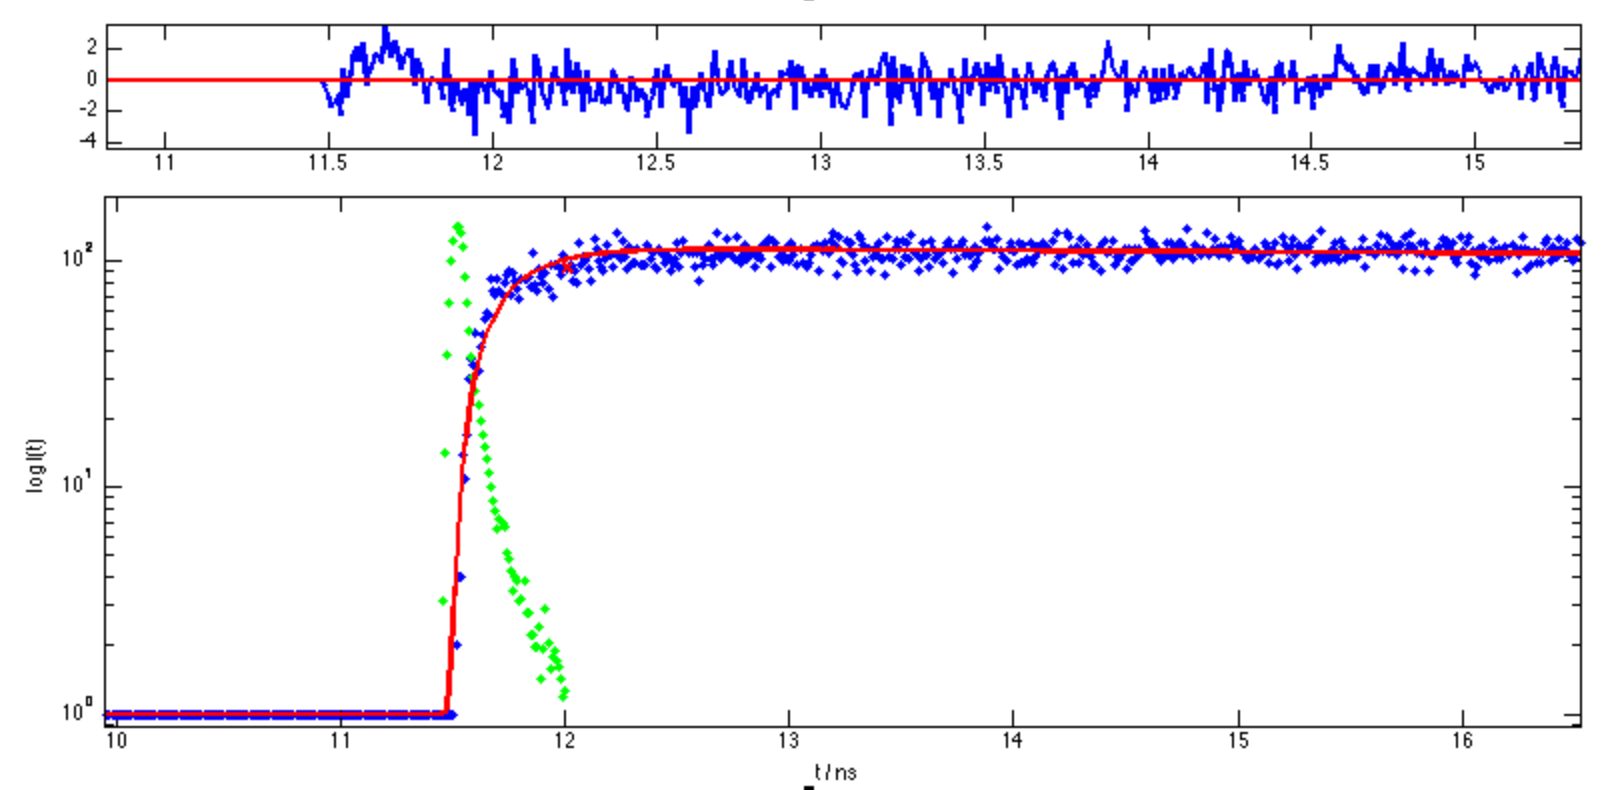
\includegraphics[width=7cm]{../Pictures/Chapter_7/0_44.png}
\end{center}
\caption[]{}
\label{fig:luag_2}
\end{figure}

\begin{figure}[htbp]
\begin{center}
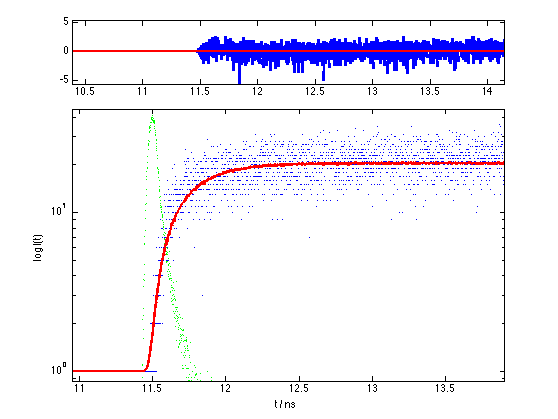
\includegraphics[width=7cm]{../Pictures/Chapter_7/luag_2735_0_13.png}
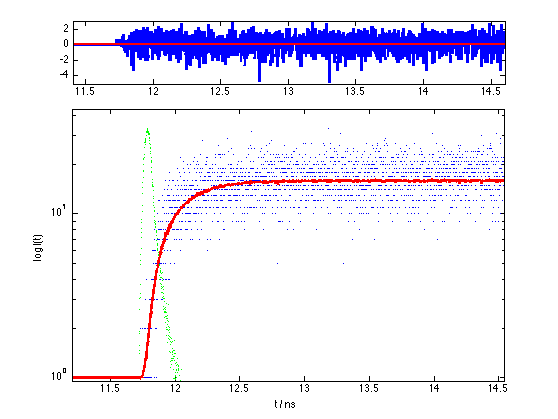
\includegraphics[width=7cm]{../Pictures/Chapter_7/luagpr.png}
\end{center}
\caption[]{}
\label{fig:pr_bgo}
\end{figure}

\begin{table}[h]
\begin{center}
\begin{tabular}{llll}
Crystal  & $\tau _{r}$ & $\tau _{d, 1}$ & $\tau _{d, 1}$ \\
LuAG:Ce (0.08$\%$)    & 280_{-51}^{+52} ps         & 40.5_{-0.7}^{+0.9} ns  & longer\\
LuAG:Ce (0.13$\%$)    & 270_{-54}^{+54} ps         & 39_{-0.7}^{+0.9} ns & longer\\ 
LuAG:Ce (0.44$\%$)     & 190_{-40}^{+45} ps         & 37_{-0.8}^{+0.8} ns  & longer \\ 
LuAG:Ce (0.5$\%$)      & 212_{-45}^{+45} ps         & 10_{-0.3}^{+0.4} ns  & longer \\ 
LuAG:Pr & 190_{-50}^{50} ps         & 38_{-0.8}^{+0.8} ns & 
\end{tabular}
\end{center}
\label{table:table}
\end{table}

\subsection{Limitations}

The setup is limited due to two constraints: the time resolution of the detection system and accumulation times. 
This two problems are intimately related on side, since given a certain time resolution, it is necessary to accumulate for longer times to reduce the incertitude on the extracted parameter. This is not always possible for crystals used in high energy and medical physics, because the long values of time constants requires longer time windows and bigger binnings.
Moreover attention should be paid for very fast rise times, if the constant extracted is close to the measured response, as it is the case for many samples object of this study. In this case deconvolution is less reliable.
This goes for the statistical error, but the limited resolution of the detection system influences the way the time profiles can be extracted. 
Indeed, as briefly explained in the previous chapter, the way parameters are extracted in canonical fluorescence analysis are strictly model dependent. That is, accurate distinction between one or multi component exponential can be hard.
This means that only qualitative analysis can be done, comparing rise times of different samples in different condition, obtaining effective parameters usually sufficient for any practical application.
More difficult is define quantities related to specific processes in the lattice, unless a thorough wavelength analysis is performed, see for example \cite{Belsky2013}.

A third limitation is the excitation energy. As explained in the previous chapter there is a non negligible contribution coming from high energy excitation, especially form Cerenkvo photons collected. With VUV this information is not accessible. On the other hand in this geometry it is possible to neglect the spread given by photon extraction, and compare this with respect to higher energy excitation. 

\subsection{Discussion}
As already stated, the crystal measured can be grossly divided in two groups.
The first contains BGO and CeF$_{3}$, that is two intrinsic and self activated scintillators and lutetium ortho silicate with Cerium doping. They have fast ($<$40 ps) rise times, indicating that the excited states are rapidly created after an ionization event.
A second group contains the doped Garnets, LuAG:Ce and LuAG:Pr. They have slower rise times due to processes that delay the transport of charge carriers to the activator atom.

Considering the limits of the setup presented before, these results are not trivial to interpret.
It is possible to consider two lines of analysis to explain the results 
\begin{itemize}
\item dopant concentration
\item competitive processes due to lattice characteristics
\end{itemize}
A first look at the result may suggest a correlation between dopant concentration and rise time. In particular more available cerium sites for scintillation entail faster transfer to excited states and thsu faster rise times, save quenching effects.

No information about Cerium concentration in the LSO samples measured was available. Nevertheless considering the standard dopant concentration for industrial crystal from manufacturers, the concentration is likely to be around 1$\%$ molar. 
Intrinsic scintillators seem to show a faster rise times, indicating that the transfer efficiency at the level of rise times to the luminescence centers is fast. For example in the case of CeF$_{3}$ the molar concentration of Cerium centers is 1. Based on the data obtained, though, there is no evidence that intrinsic scintillator are faster than extrinsic in the LSO group, which could be expected based on a dopant concentration dependance. It should be noted that this values are at the very limit of the detection system, so statistically less accurate.

On the other hand perfectly known is the Cerium concentration for the Garnet samples. 
The Garnet samples belong to different batches, so caution should be considered when a comparative analysis is performed, since growth parameters can differ significatively. Based on the error of the measurement though it is not possible to conclude that crystals with low percentage of doping show slower rise times, even if the tendency shown deserves a better understanding. Indeed the 0.08$\%$ and the 0.13 $\%$ Cerium doped samples present the slower rise times for the Garnet group, and a measurement campaing changing the dopant concentration over a wide range of dopings could be resolutive, see for example the non conclusive study made on LaBr$_{3}$ in \cite{Moses2004}.

It is necessary to consider also a "horizontal" analysis based on the very different lattices, dopants and scintillation mechanism of the samples measured. In LuAG crystals, for example, an important role is played by excitonic transition and only a wavelength based analysis can reveal possible differences, see for example \cite{Belsky2013}.
It is clear that differences between Cerium doped LSO and LuAG samples can not be explained solely based on dopant concentration difference.

\subsection{Perspectives}
Intrinsic limitations of the setup do not allow for a definitive assessment of rise time properties. Given the high error associated with measurement, the biggest effort should be reserved to the improvement of the accuracy.

In order to achieve that, a first idea is to tackle the statistical limitations due to the number of samples analyzed. An extensive campaign should be performed with different crystal species, alternating combinations of lattice, dopants and concentration. This would be very time-demanding.

Time constraints are the main limitations for a complete wavelength analysis, especially in the case of crystals with different scintillating components. This is interesting for Garnets, for example, LaBr$_{3}$ or more complex insulators like LiYF$_{4}$.

The most important improvement, though could come from the detection method. There are two ways of achieving this: improving the IRF of the detection system or exploit a classical approach of fluorescence analysis, frequency mixing. The IRF of the detection system depends mainly on the stop detector and it has some lower limit at a few tens of ps. This makes the analysis of processes at the pico second scale not possible.
Frequency mixing approach on the other hand relies on second order processes in non linear crystals, so to rely less on read out electronics. The problems concerns mainly feasibility for slow crystals, since these techniques require fast and bright emissions.